%!TEX root = paper.tex
%related.tex

\section{Related work}
\label{sec:related}

\subsection{Privacy and Government}
This work falls within a line of research that investigates the balance of power between citizens and the state. In~\cite{laskowskigovernment}, we investigated the application of surveillance technology by a government that wishes to remain in power.  Our main takeaway was that enhanced surveillance technology increases incentives for abuse. 

In a similar vein, Goh provides a model of a government that may employ surveillance to lower the risk of a terrorist attack \cite{goh2015prosperity}.  Greater surveillance carries an increased risk that citizens will learn of its existence, which increases the risk that the government loses power.  Goh finds that a rational government will employ less surveillance when citizens value their privacy more, but autocratic governments will employ more surveillance than democratic ones.

A larger literature examines the relationship between citizens and the state in general.  Downs~\cite{downs1957economic} provides a model of political competition based on a continuum of political preferences, extending Hoteling's study of horizontal differentiation~\cite{press39hotelling}.  Further studies model the process by which governments are overthrown.  Ginkel and Smith~\cite{ginkel1999so} consider factors that determine the probability of revolution in a repressive regime.  Lohmann~\cite{lohmann1994dynamics} describes the potential overthrow of a government through an informational cascade model. Kuran~\cite{kuran1989sparks} attempts to explain why revolutions often take the world by surprise with a game theoretic model of political change.  These studies do not consider the effects of privacy in determining political outcomes.

\subsection{Privacy and Firms}

Privacy also affects the relationship between citizens and firms, and several strands of research shed light on this topic (Acquisti provides a survey \cite{acquisti2010economics}).  Privacy can be seen in the classic literature on information economics as an information imbalance between a principal and an agent.  Moral hazard models assume that an agent's actions are not directly observable and the focus is on aligning incentives through contracting \cite{holmstrom1979moral}\cite{stiglitz1981credit}.  In models of adverse selection, agent types are private and certain types are driven out of a market because the principal cannot distinguish between them \cite{akerlof1995market}.  In signaling games, agents may engage in costly actions to signal their private type for economic gain \cite{spence1973job}.  None of these settings correspond to our focus on privacy as protecting a marginalized group.  Furthermore, models in this literature are usually neoclassical in the sense that privacy is an obstacle to maximizing welfare. 

An emerging body of privacy research models the behavior of consumers that participate in two different markets in sequence.  Firms in one market learn about consumers based on their purchase decisions and may be allowed to sell this information to firms in the second market.  A common theme in this literature is the fact that outcomes depend on whether consumers are myopic, considering each purchase decision without regard for how it will affect future purchases, or fully sophisticated.  In \cite{johnsoncaviar}, we found that when consumers are myopic, firms benefit greatly, but consumer surplus is also reduced. When we assume that consumers are strategic, consumers are better off, but firms fare worse.  In a similar vein, Acquisti and Varian look at a single monopolist that sells two goods in series \cite{acquisti2005conditioning}.  Taylor examines the case of two firms when consumer valuations for each good can take on two values, but these valuations are not perfectly correlated with each other \cite{taylor2004consumer}.  Information sharing may increase or decrease consumer surplus and welfare, depending on the demand specification.  

Other studies provide further examples of scenarios in which privacy is welfare-enhancing.  Hermalin and Katz discuss insurance markets and investments in information gathering \cite{hermalin2006privacy}.  Taylor considers a scenario in which collecting information about customers is costly and firms may overinvest in this activity \cite{taylor2003privacy}.  Hann et al. argue that unsolicited marketing imposes negative costs on consumers in the absence of privacy regulation \cite{hann2008consumer}.

A final literature studies privacy through the lens of mechanism design.  Calzolari and Pavan describe a framework in which firms may offer arbitrary contracts to users \cite{calzolari2006optimality}.   A set of recent papers have pioneered the use of differential privacy as a solution concept \cite{pai2013privacy}.  In these models, agents must be approximately truthful to the mechanism and cannot change the outcome by very much if they lie or refuse to participate.  Protecting privacy is not the focus of these models, since the solution concept begins with an assumption that agents don't hide information.

In contrast to the studies we mention, which treat privacy as a binary parameter, our work distinguishes four distinct types of privacy, which are inspired by technologies and legal debate.  We further apply our model to explore the effects of privacy on divisive laws.

\subsection{Technological Features of Privacy}

Citizens that engage in behavior that is forbidden by a law may employ privacy-enhancing technologies, such as the anonymizing Tor network~\cite{dingledine2003privacy}.  Sweeney defines a notion, k-anonymity, to measure the anonymity provided by a particular dataset \cite{sweeney2002k}. Technologies also mediate the enforcement of laws.  The ability of a government to identify law-breakers is enhanced through techniques like dataset aggregation\cite{acquisti2009predicting}.  An ongoing debate surrounds the use of these and other technologies, in contexts ranging from ethics\cite{lyon2002surveillance,diffie2010privacy}, to law\cite{landau2009,landau2013making,landau2014,Bankston14}, to security-relevant effectiveness~\cite{schneier2013oppression%,schneier2013surveillance
}.  While our model abstracts from these details, we will use it to explore the impact of technologically-based privacy.


\subsection{Polarization}
Most voters in the United States are overwhelmingly moderate in their policy positions\cite{layman2006party}.   Nevertheless, the United States Congress has passed a number of divisive laws, many of which have been challenged and overturned by the US Supreme Court.  Divisive laws have also been passed in European countries, including those against face covering, pejoratively dubbed ``burka bans.''


\begin{figure}[htbp]
\begin{center}
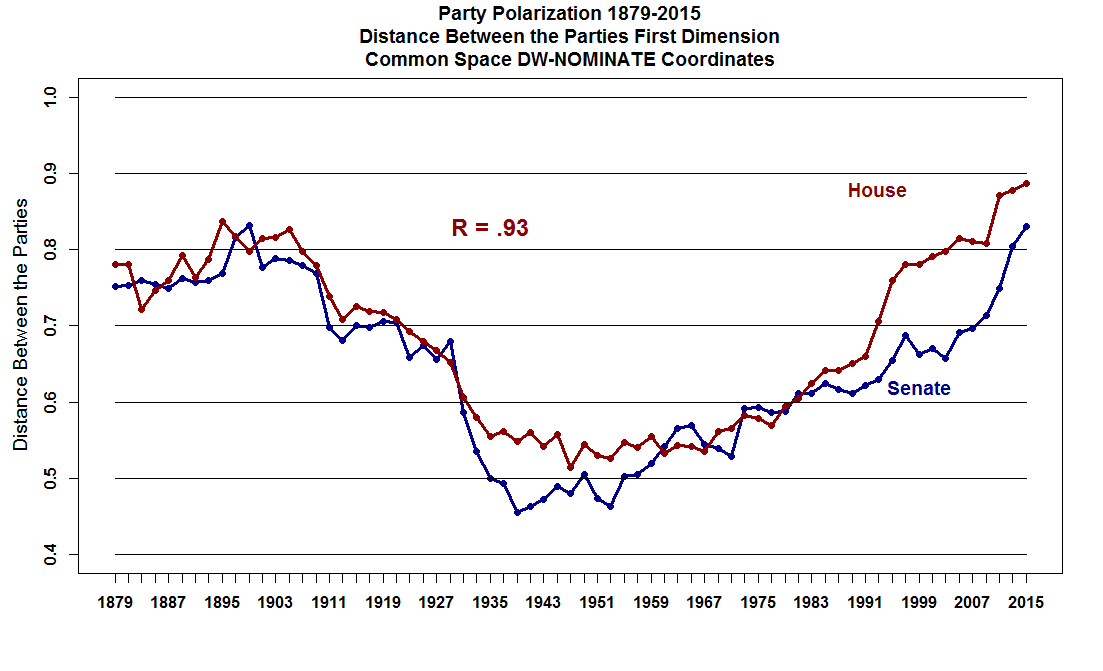
\includegraphics[width=0.4\textwidth]{figs/polar_house_and_senate_46-115_july_11}
\caption{{\bf Polarization Trends in the US Congress}}
\label{fig:uscongress}
\end{center}
\end{figure}




The United States congress in particular has become increasingly polarized over the last 40 years (see Figure \ref{fig:uscongress}).  Today, members of congress exhibit a distinctly bimodal distribution in terms of political preferences, as seen in \ref{fig:partisonship}.  Researchers have posited a number of reasons for this phenomenon \cite{barber2015causes}\cite{poole1984polarization}, ranging from a polarized electorate, to southern realignment, to gerrymandering, to the evolution of modern primary elections, to economic inequality, to money in politics, to the media environment, or to congress-based factors such as congressional rule changes, majority party agenda control, party pressures, teamsmanship, or the breakdown of bipartisan norms.  All of these issues are discussed in~\cite{poole1984polarization}.
More culturally-specific theories involving authoritarianism are also prevalent \cite{hetherington2009authoritarianism}.

\begin{figure}[htbp]
\begin{center}
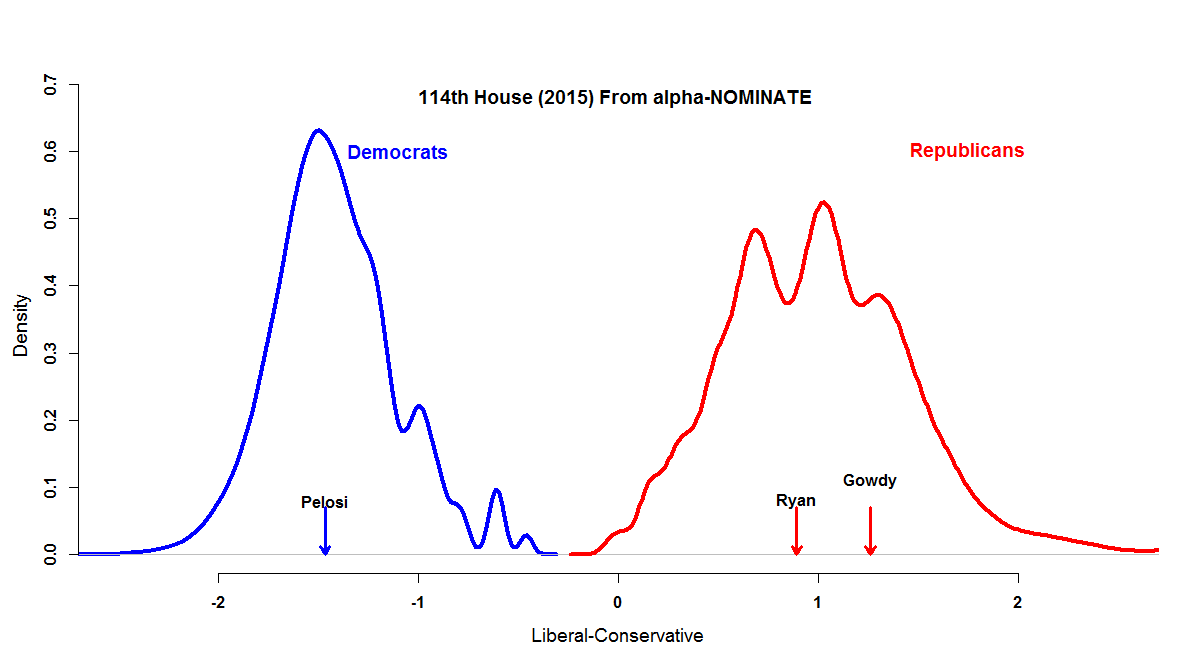
\includegraphics[width=0.4\textwidth]{figs/alpha_House_114_Histogram_8_January_2016}
\caption{{\bf Partisonship in the US House of Representatives}}
\label{fig:partisonship}
\end{center}
\end{figure}


%; and there is a remarkably close correlation between economic
%inequality and polarization in the United States~\cite{mccarty2006polarized}.  See Figure \ref{fig:inequality}.

%\begin{figure}[htbp]
%\begin{center}
%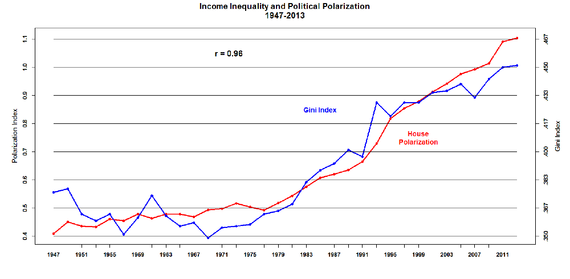
\includegraphics[width=0.4\textwidth]{figs/8141eb7a0}
%\caption{{\bf Polarization versus Income Inequality}}
%\label{fig:inequality}
%\end{center}
%\end{figure}


A more economically-driven explanation derives from the notion of information cascades. An information cascade occurs when people receive a noisy informational signal and observe the behavior of friends and colleagues to inform decision-making.  Although agents are individually rational, they may find it optimal to rely on the information they derive from previous agents, ignoring their private signals \cite{bikhchandani1992theory}.

The notion that people exhibit herding behavior in predictable circumstances has been around for decades \cite{shiller1995conversation}.  For example, researchers at Iowa State University conducted 259 interviews with farmers who had largely refused offers to adopt drought-resistant seed corn during the Great Depression and Dust Bowl.  They found that the slow rate of adoption was due to ``how farmers valued the opinion of their friends and neighbors instead of the word of a salesman''\cite{beal1957diffusion}.


We include a notion of influenced behavior in our model as a way to describe the polarization of society.  Our model does not mandate that citizens consider how a law affects other citizens, but merely allows it.  This allowance appears justified by the observation that the United States has a legislative system that is organized like Figure \ref{fig:partisonship}, while it has an electorate that is more like Figure \ref{fig:voters}.





\begin{figure}[htbp]
\begin{center}
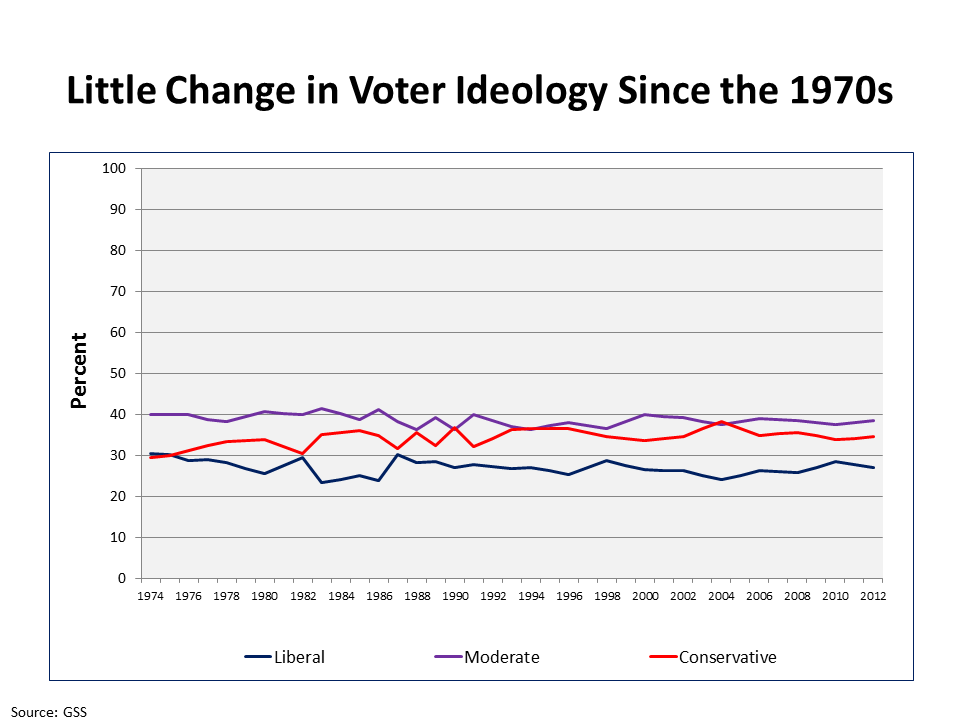
\includegraphics[width=0.4\textwidth]{figs/polarization2}
\caption{{\bf Long Term Trends in US Voter Ideology}}
\label{fig:voters}
\end{center}
\end{figure}





